% intuitive
\section*{Background}
\addcontentsline{toc}{section}{\protect\numberline{}{Background}}

%\paragraph{Context}
% domain
The discovery of the DNA structure\citep{watson1953structure} was followed by
developing sequencing technologies that enabled acquiring genomic data in a
linear format, similar to human text and speech. With the development of
sequencing technologies, the amount and complexity of the available genomic data
bacame not only intractable by hand, but also challenging for computer analysis.
Sequence alignment has been a core problem in computational biology for the last
half-century with a multitude of applications. In this thesis I propose a novel
principled approach to sequence alignment and search, and demonstrate its
superior performance on genomic data (including metagenomic data).

\paragraph{Alignment problem}
% problem statements
We consider the problem of pairwise sequence alignment in the context of genomic
data: given two DNA sequences, one has to be aligned to the other. It would have
been a rather trivial task if the alignment would be perfect. Nevertheless, the
real data contains both biological variation and technical errors resulting from
evolution and the sequencing process. A common intuitive and robust assumption
is that an alignment with a minimal number of single-letter edits
(substitutions, insertions and deletions) is the most plausable explainationo of
the divergence of both sequences from an unknown common ancestor.

% alignment types
\begin{figure}[t]  %\begin{floatingfigure}[l]{0.5\textwidth}
    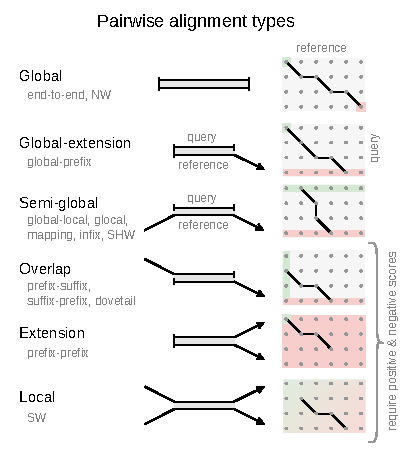
\includegraphics[width=0.5\textwidth]{alignment-types}
	\caption[Alignment types]{Alignment types.}
    \label{fig:alignment-types}
\end{figure}
Two sequences can be aligned in multiple ways (\cref{fig:alignment-types}). In
this thesis we focus on global and semi-global alignment types only. If both
sequences have to be aligned end to end, we look for a \emph{global alignment}
whose minimal number of edits is known as \emph{edit distance}. If we instead
search for an occurance of a query sequence within a reference sequence, we
allow the alignment to start and end at any reference locations in a
\emph{semi-global} alignment (also called approximate/fuzzy string search
outside computational biology).

\paragraph{Sequencing}
Genomic (DNA, RNA) sequencing is a technology that takes genetic material and
produces a data file with a set of sequences. Each sequence from a new
biological sample can be compared to a reference genome (if such is available)
in order to identify mutations, quantify expression per gene, and many other
types of analysis. To figure out which part of the reference each sequence most
probably originates from, it should first be semi-globally aligned to the
reference.

\paragraph{Dynamic programming}
The first efficient solution for global alignment, known as the Needleman-Wunsch
algorithm, got developed around~\citeyear{vintsyuk1968speech}~
\cite{vintsyuk1968speech,needleman1970general}. This algorithm is based on the
then newly-developed dynamic programming (DP) technique~\cite{bellman1954theory}
of splitting a task into overlapping subtasks and reusing their solutions. Thus,
combining optimal alignments of prefixes of the sequences, allows to choose an
optimal solution for only quadratic time with the sequences length, despite of
the exponential number of candidates.

Since semi-global alignment requires not only aligning but also determining a
starting position in the reference, an application of the same DP approach came
a decade later~\cite{sellers1980theory,smith1981identification} and took
$\Oh(nm)$ to align a single query of length $n$ to a reference of length $m$. It
is highly redundant to explore the whole reference for each alignment, so
various data structures were suggested that can be precomputed to index the
reference, and then reuse this index to quickly align multiple query sequences
~\citeyear{pearson1988improved}~\cite{pearson1988improved} and has become
central to read alignment of high-throughput sequencing.

Considering the subtasks of aligning one prefix to another prefix remains a main
the domain in which most appoaches to optimal alignment work, regardless of
using DP.

\paragraph{Optimal alignment}

An important factor for the development of the sequencing algorithms is the
technological advancement~\cite{alser2021technology}. One possible reason is the
combination of massive new data and advancement in computation hardware allowing
for various kinds of parallelization.
%Thus the advancements with bit-parallel algorithms (CITE Myears, Mikko).

\paragraph{Metagenomics}
% graph references for semi-global
The development of high-throughput sequencing technologies lead to higher
amounts of cheaper data. The abundance of data enabled the assembly of richer
references that capture biological variation from different individuals and
species. In particular, the last decade saw the increased development of graph
references that compactly represent a whole set of genomes (a metagenome) as
paths. Semi-global alignment of de novo sequences on such graphs produces more
accurate alignments than on linear references.

\paragraph{Applications}

% parallelization
% sketches

% Optimal DP-based approaches
\paragraph{Optimal alignment}
Current optimal alignment algorithms reach the impractical $\Oh(nm)$ runtime
that has been shown to be a lower bound for the worst-case edit distance
computation~\cite{backurs2015edit}. In this light, approaches for improving the
efficiency of optimal alignment have taken advantage of specialized features of
modern CPUs to improve the practical runtime of the Smith-Waterman dynamic
programming (DP) algorithm~\cite{smith_comparison_1981} considering all possible
starting nodes. These use modern SIMD instructions (\eg
\vg~\cite{garrison_variation_2018} and \pasgal~\cite{jain_accelerating_2019}) or
reformulations of edit distance computation to allow for bit-parallel
computations in \graphaligner \footnote{We refer as \bitparallel to to the
bit-parallel DP algorithm implemented in \graphaligner tool
\cite{rautiainen_bitparallel_2019}.}~\cite{rautiainen_bitparallel_2019}. Many of
these, however, are designed only for specific types of genome graphs, such as
{\itshape de Bruijn}
graphs~\cite{liu_debga_2016,limasset2019toward} and
variation graphs~\cite{garrison_variation_2018}. A compromise often made when
aligning sequences to cyclic graphs using algorithms reliant on directed acyclic
graphs involves the computationally expensive ``DAG-ification'' of graph
regions~\cite{kavya_sequence_2019,garrison_variation_2018}.

\paragraph{Seed-and-Extend}
Since optimal alignment is often intractable, many aligners use heuristics, most
commonly the \emph{seed-and-extend}
paradigm~\cite{altschul_basic_1990,langmead_fast_2012,li_fast_2009}. In this
approach, alignment initiation sites (\emph{seeds}) are determined, which are
then \emph{extended} to form the \emph{alignments} of the query sequence. The
fundamental issue with this approach, however, is that the seeding and extension
phases are mostly decoupled during alignment. Thus, an algorithm with a provably
optimal extension phase may not result in optimal alignments due to the
selection of a suboptimal seed in the first phase. In cases of high sequence
variability, the seeding phase may even fail to find an appropriate seed from
which to extend.

\paragraph{Known limitations}

Quadratic optimal for semi-global

In its general case, it is not solvable for strictly subquadratic time which is
often prohibitively slow. Faster approximate algorithms are instead used in
practice. We employ the \A informed search algorithm in order to design an
optimal algorithm that scales subquadratically for related sequences.
